\documentclass{standalone}
\usepackage{tikz}
\usetikzlibrary{patterns, positioning}
\usetikzlibrary{shapes.misc}
\usepackage[outline]{contour}
\contourlength{1.5pt} 


\begin{document}
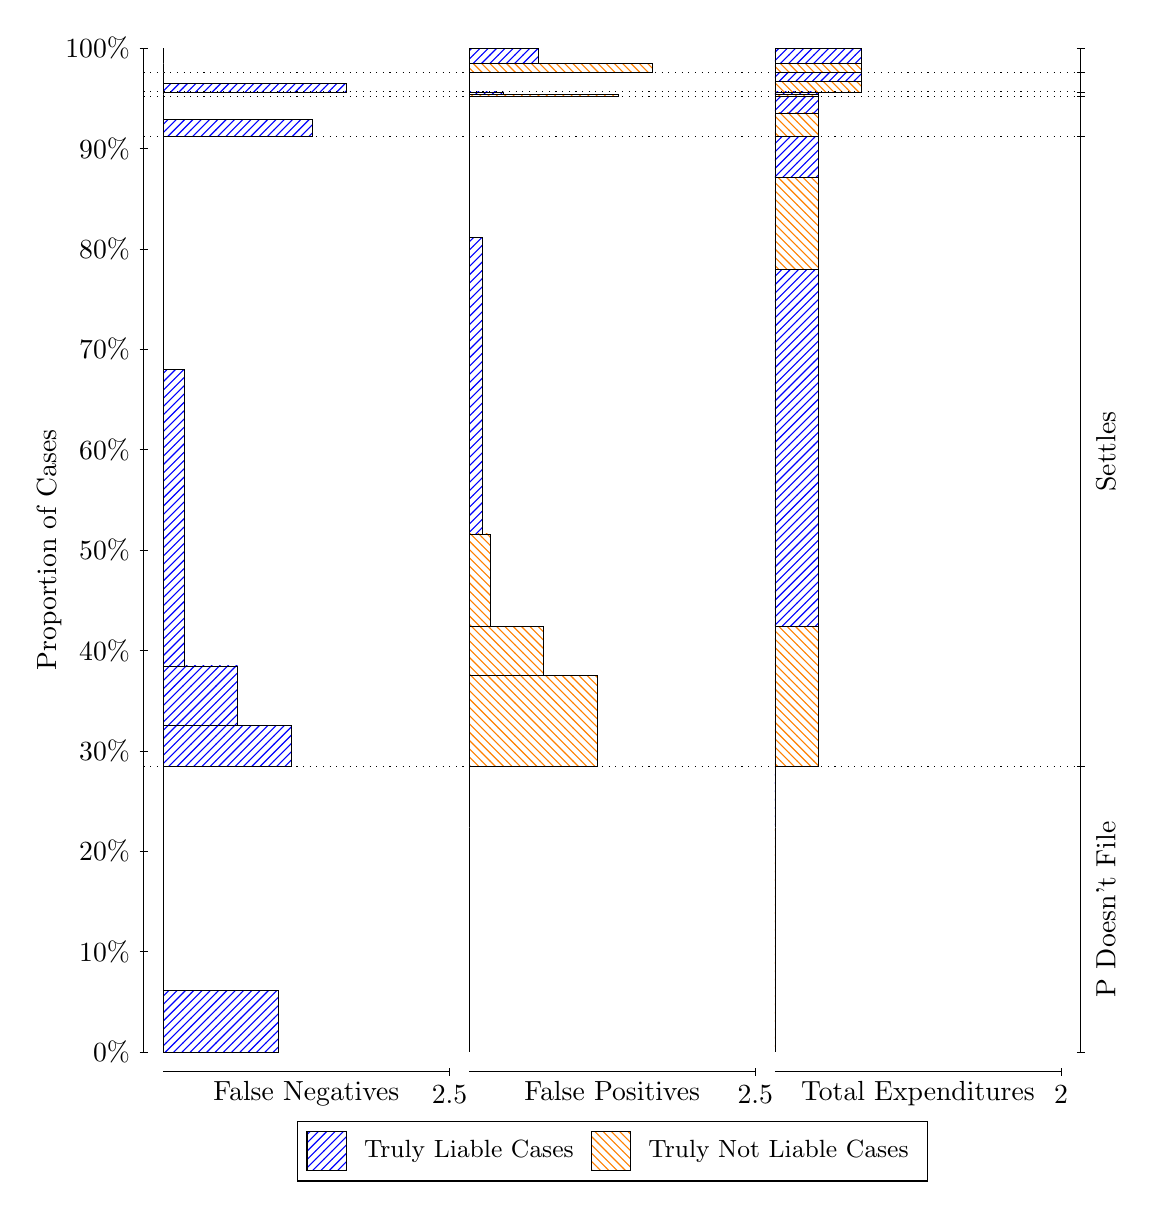
\begin{tikzpicture}
\draw[black, very thin] (1.5,1.75) -- (1.5,14.5);
\node[rotate=90, text=black, anchor=center] at (0.3, 8.125) {Proportion of Cases};
\draw[black, very thin] (1.45,1.75) -- (1.55,1.75);
\node[text=black, anchor=east] at (1.45, 1.75) {0\%};
\draw[black, very thin] (1.45,3.025) -- (1.55,3.025);
\node[text=black, anchor=east] at (1.45, 3.025) {10\%};
\draw[black, very thin] (1.45,4.3) -- (1.55,4.3);
\node[text=black, anchor=east] at (1.45, 4.3) {20\%};
\draw[black, very thin] (1.45,5.575) -- (1.55,5.575);
\node[text=black, anchor=east] at (1.45, 5.575) {30\%};
\draw[black, very thin] (1.45,6.85) -- (1.55,6.85);
\node[text=black, anchor=east] at (1.45, 6.85) {40\%};
\draw[black, very thin] (1.45,8.125) -- (1.55,8.125);
\node[text=black, anchor=east] at (1.45, 8.125) {50\%};
\draw[black, very thin] (1.45,9.4) -- (1.55,9.4);
\node[text=black, anchor=east] at (1.45, 9.4) {60\%};
\draw[black, very thin] (1.45,10.675) -- (1.55,10.675);
\node[text=black, anchor=east] at (1.45, 10.675) {70\%};
\draw[black, very thin] (1.45,11.95) -- (1.55,11.95);
\node[text=black, anchor=east] at (1.45, 11.95) {80\%};
\draw[black, very thin] (1.45,13.225) -- (1.55,13.225);
\node[text=black, anchor=east] at (1.45, 13.225) {90\%};
\draw[black, very thin] (1.45,14.5) -- (1.55,14.5);
\node[text=black, anchor=east] at (1.45, 14.5) {100\%};

\draw[black, very thin] (13.4,1.75) -- (13.4,14.5);
\draw[black, very thin] (13.35,1.75) -- (13.45,1.75);
\node[anchor=west] at (13.35, 1.75) {};
\draw[black, very thin] (13.35,5.375) -- (13.45,5.375);
\node[anchor=west] at (13.35, 5.375) {};
\draw[black, very thin] (13.35,13.378) -- (13.45,13.378);
\node[anchor=west] at (13.35, 13.378) {};
\draw[black, very thin] (13.35,13.89) -- (13.45,13.89);
\node[anchor=west] at (13.35, 13.89) {};
\draw[black, very thin] (13.35,13.944) -- (13.45,13.944);
\node[anchor=west] at (13.35, 13.944) {};
\draw[black, very thin] (13.35,14.187) -- (13.45,14.187);
\node[anchor=west] at (13.35, 14.187) {};
\draw[black, very thin] (13.35,14.5) -- (13.45,14.5);
\node[anchor=west] at (13.35, 14.5) {};

\draw[black, very thin, pattern color=blue, pattern=north east lines] (1.75,1.75) rectangle (3.2033,2.5273);
\draw[black, very thin, pattern color=orange, pattern=north west lines] (1.75,2.5273) rectangle (1.75,5.375);
\draw[black, very thin, pattern color=blue, pattern=north east lines] (1.75,5.375) rectangle (3.3729,5.8947);
\draw[black, very thin, pattern color=blue, pattern=north east lines] (1.75,5.8947) rectangle (2.6947,6.6538);
\draw[black, very thin, pattern color=blue, pattern=north east lines] (1.75,6.6538) rectangle (2.0164,10.422);
\draw[black, very thin, pattern color=orange, pattern=north west lines] (1.75,10.422) rectangle (1.75,13.378);
\draw[black, very thin, pattern color=blue, pattern=north east lines] (1.75,13.378) rectangle (3.6393,13.593);
\draw[black, very thin, pattern color=orange, pattern=north west lines] (1.75,13.593) rectangle (1.75,13.89);
\draw[black, very thin, pattern color=orange, pattern=north west lines] (1.75,13.89) rectangle (1.75,13.911);
\draw[black, very thin, pattern color=blue, pattern=north east lines] (1.75,13.911) rectangle (1.75,13.944);
\draw[black, very thin, pattern color=blue, pattern=north east lines] (1.75,13.944) rectangle (4.0753,14.05);
\draw[black, very thin, pattern color=orange, pattern=north west lines] (1.75,14.05) rectangle (1.75,14.187);
\draw[black, very thin, pattern color=orange, pattern=north west lines] (1.75,14.187) rectangle (1.75,14.304);
\draw[black, very thin, pattern color=blue, pattern=north east lines] (1.75,14.304) rectangle (1.75,14.5);
\draw[black, very thin, pattern color=orange, pattern=north west lines] (5.6333,1.75) rectangle (5.6333,4.5977);
\draw[black, very thin, pattern color=blue, pattern=north east lines] (5.6333,4.5977) rectangle (5.6333,5.375);
\draw[black, very thin, pattern color=orange, pattern=north west lines] (5.6333,5.375) rectangle (7.2562,6.5301);
\draw[black, very thin, pattern color=orange, pattern=north west lines] (5.6333,6.5301) rectangle (6.578,7.1571);
\draw[black, very thin, pattern color=orange, pattern=north west lines] (5.6333,7.1571) rectangle (5.8998,8.3305);
\draw[black, very thin, pattern color=blue, pattern=north east lines] (5.6333,8.3305) rectangle (5.8029,12.099);
\draw[black, very thin, pattern color=blue, pattern=north east lines] (5.6333,12.099) rectangle (5.6333,13.378);
\draw[black, very thin, pattern color=orange, pattern=north west lines] (5.6333,13.378) rectangle (5.6333,13.675);
\draw[black, very thin, pattern color=blue, pattern=north east lines] (5.6333,13.675) rectangle (5.6333,13.89);
\draw[black, very thin, pattern color=orange, pattern=north west lines] (5.6333,13.89) rectangle (7.5227,13.911);
\draw[black, very thin, pattern color=blue, pattern=north east lines] (5.6333,13.911) rectangle (6.0693,13.944);
\draw[black, very thin, pattern color=orange, pattern=north west lines] (5.6333,13.944) rectangle (5.6333,14.081);
\draw[black, very thin, pattern color=blue, pattern=north east lines] (5.6333,14.081) rectangle (5.6333,14.187);
\draw[black, very thin, pattern color=orange, pattern=north west lines] (5.6333,14.187) rectangle (7.9587,14.304);
\draw[black, very thin, pattern color=blue, pattern=north east lines] (5.6333,14.304) rectangle (6.5053,14.5);
\draw[black, very thin, pattern color=orange, pattern=north west lines] (9.5167,1.75) rectangle (9.5167,4.5977);
\draw[black, very thin, pattern color=blue, pattern=north east lines] (9.5167,4.5977) rectangle (9.5167,5.375);
\draw[black, very thin, pattern color=orange, pattern=north west lines] (9.5167,5.375) rectangle (10.062,7.1571);
\draw[black, very thin, pattern color=blue, pattern=north east lines] (9.5167,7.1571) rectangle (10.062,11.685);
\draw[black, very thin, pattern color=orange, pattern=north west lines] (9.5167,11.685) rectangle (10.062,12.858);
\draw[black, very thin, pattern color=blue, pattern=north east lines] (9.5167,12.858) rectangle (10.062,13.378);
\draw[black, very thin, pattern color=orange, pattern=north west lines] (9.5167,13.378) rectangle (10.062,13.675);
\draw[black, very thin, pattern color=blue, pattern=north east lines] (9.5167,13.675) rectangle (10.062,13.89);
\draw[black, very thin, pattern color=orange, pattern=north west lines] (9.5167,13.89) rectangle (10.062,13.911);
\draw[black, very thin, pattern color=blue, pattern=north east lines] (9.5167,13.911) rectangle (10.062,13.944);
\draw[black, very thin, pattern color=orange, pattern=north west lines] (9.5167,13.944) rectangle (10.607,14.081);
\draw[black, very thin, pattern color=blue, pattern=north east lines] (9.5167,14.081) rectangle (10.607,14.187);
\draw[black, very thin, pattern color=orange, pattern=north west lines] (9.5167,14.187) rectangle (10.607,14.304);
\draw[black, very thin, pattern color=blue, pattern=north east lines] (9.5167,14.304) rectangle (10.607,14.5);
\draw[black, dotted] (1.5,5.375) -- (13.4,5.375);
\draw[black, dotted] (1.5,13.378) -- (13.4,13.378);
\draw[black, dotted] (1.5,13.89) -- (13.4,13.89);
\draw[black, dotted] (1.5,13.944) -- (13.4,13.944);
\draw[black, dotted] (1.5,14.187) -- (13.4,14.187);
\draw[black, very thin] (1.75,1.5) -- (5.3833,1.5);
\node[text=black, anchor=north] at (3.5667, 1.5) {False Negatives};
\draw[black, very thin] (5.3833,1.45) -- (5.3833,1.55);
\node[text=black, anchor=north] at (5.3833, 1.45) {2.5};

\draw[black, very thin] (5.6333,1.5) -- (9.2667,1.5);
\node[text=black, anchor=north] at (7.45, 1.5) {False Positives};
\draw[black, very thin] (9.2667,1.45) -- (9.2667,1.55);
\node[text=black, anchor=north] at (9.2667, 1.45) {2.5};

\draw[black, very thin] (9.5167,1.5) -- (13.15,1.5);
\node[text=black, anchor=north] at (11.333, 1.5) {Total Expenditures};
\draw[black, very thin] (13.15,1.45) -- (13.15,1.55);
\node[text=black, anchor=north] at (13.15, 1.45) {2};

\node[text=black, centered, rotate=90] at (13.72, 3.5625) {\contour{white}{P Doesn't File}};
\node[text=black, centered, rotate=90] at (13.72, 9.3763) {\contour{white}{Settles}};





\draw (7.449999999999999,1.5) node[draw=none] (baseCoordinate) {};
\begin{scope}[align=center]
        \matrix[scale=0.5, draw=black, below=0.5cm of baseCoordinate, nodes={draw}, column sep=0.1cm]{
            \node[rectangle, draw, minimum width=0.5cm, minimum height=0.5cm, pattern color=blue, pattern=north east lines] {}; &
            \node[draw=none, font=\small, text=black] (B) {Truly Liable Cases}; &
            \node[rectangle, draw, minimum width=0.5cm, minimum height=0.5cm, pattern color=orange, pattern=north west lines] {}; &
            \node[draw=none, font=\small, text=black] (B) {Truly Not Liable Cases}; \\
            };
\end{scope}

\end{tikzpicture}
\end{document}